% Double-anonymous review copy for FORGE 2027 (co-located with ICSE 2027,
% Dublin). FORGE 2027 requires the IEEE conference template
% (\documentclass[10pt,conference]{IEEEtran}, no compsoc/compsocconf).
% Shares every section file with main.tex; this file only differs in the
% anonymized author block and artifact link. Do not edit content sections
% here -- edit the shared .tex files instead. Restore main.tex's real
% \author block for the camera-ready version after acceptance.
\documentclass[10pt,conference]{IEEEtran}

\usepackage{graphicx}
\usepackage{amsmath}
\usepackage{hyperref}
\usepackage{booktabs}
\usepackage{tabularx}
\hypersetup{pdfauthor={},pdftitle={Coverage-Free Fuzzing: LLM-Guided Refinement of Grammar-Based Test Generators}}

% Anonymized artifact mirror -- do not point this at the real GitHub URL,
% it deanonymizes this submission.
\newcommand{\artifacturl}{https://anonymous.4open.science/r/agentic-grammar-fuzzing-6177/}

\title{Coverage-Free Fuzzing: LLM-Guided Refinement of Grammar-Based Test Generators}

\author{
\IEEEauthorblockN{Anonymous Author(s)}
\IEEEauthorblockA{Submission under double-anonymous review}
}

\begin{document}

\maketitle

\begin{abstract}
Property-based testing tools such as Hypothesis can turn a formal grammar
into a generator of syntactically valid inputs, but the generator itself is
typically static: hand-tuned once and reused unchanged for the rest of a
fuzzing campaign. We study whether a large language model (LLM), given only
a formal grammar and parser-level feedback -- with no coverage
instrumentation -- can iteratively refine such a generator. We build a fully
black-box pipeline targeting the cJSON parser (pinned at v1.7.19): a baseline
Hypothesis strategy derived directly from an ANTLR JSON grammar generates
inputs, a sanitizer-instrumented harness classifies each as accepted,
rejected, or crashing, and a refinement loop feeds an LLM a summary of three
observable proxy signals -- acceptance rate, the structural diversity of the
shapes produced, and the distinct rejection signatures seen -- asking it to
propose a revised generator. Every proposal is statically sandboxed
(AST-checked, import-restricted) and validated before it ever touches the
target binary. Across fifteen independent, seeded runs of up to five
refinement iterations each, LLM-guided refinement raises mean acceptance
rate from 58.2\% to 97.1\% relative to a static baseline, using no coverage
data at all. Structural fingerprints and rejection signatures are reported as
descriptive signals; because the refined arm executes more iterations, their
aggregate counts are not treated as like-for-like effects. A follow-up
ablation over which subset of this feedback the proposer sees -- counts
alone, counts with rejection signatures, or the full signal -- finds
acceptance-rate gains are broadly similar across the three conditions, with
full feedback preserving more rejection-signature diversity than counts
alone (four usable runs per condition; reported descriptively, not tested).
A pre-registered replication on a second parser, parson, with the same
proposer and design finds the opposite: refinement lowers mean acceptance
from 95.6\% to 92.4\% ($p \approx 0.024$), and no crash occurs in 25{,}500
sanitizer-instrumented executions. Every rejected input is explained: parson
accepts any bytes after a complete value, so the static baseline starts near
its ceiling, while the refined generators produce grammar-valid constructs
that parson refuses without reporting why. The acceptance proxy is thus only
as useful as the target is strict and informative about rejections. We
discuss how grammar-implementation mismatches -- for instance, duplicate
JSON object keys accepted by one parser and rejected by the other under an
identical grammar -- are themselves a source of fuzzing-relevant signal that
a purely formal grammar cannot supply, and we release the full pipeline,
harnesses, and reproducibility tooling.

\end{abstract}

\begin{IEEEkeywords}
fuzzing, grammar-based testing, property-based testing, large language models, black-box testing, software testing
\end{IEEEkeywords}

\section{Introduction}

Parsers are among the most exposed pieces of code in any system: they are
the first code to touch untrusted input, and a memory-safety bug in a parser
is directly attacker-controlled. Fuzzing -- automatically generating inputs
and observing how a target handles them -- is the standard defense, but the
two dominant families of fuzzer make different tradeoffs around structure and
feedback. Coverage-guided, mutation-based fuzzers such as AFL discover
interesting inputs by instrumenting the target and rewarding inputs that
reach new code, but for a structured format such as JSON, random byte-level
mutation of a seed corpus destroys syntactic validity far more often than it
discovers it, so most of the fuzzer's budget is spent on inputs the parser
rejects in its first few bytes. Grammar-based and property-based approaches
invert this: a generator is written directly against a grammar or schema, so
every input is syntactically valid (or deliberately near-valid) by
construction, and the fuzzer's budget goes toward exploring the target's
\emph{structural} handling of the format rather than re-discovering its
lexer. Hypothesis, the property-based testing library we build on, is one
such approach: a developer composes strategies -- generators for values of a
given shape -- that can mirror a grammar directly.

The gap is that a hand-written grammar-based generator is usually static. It
is authored once, and unless a human revisits it, it keeps producing the
same distribution of shapes for the rest of a campaign, no matter what the
target's actual behavior turns out to be. Coverage-guided fuzzers close an
analogous loop by using instrumentation feedback to reward and retain
interesting inputs; grammar-based generators typically have nothing
equivalent, because the whole appeal of generating from a grammar is that it
does not require instrumenting or even recompiling the target. This is not
a minor convenience: many realistic targets -- vendored third-party
libraries pinned at a specific commit, closed-source or license-restricted
binaries, embedded or cross-compiled parsers -- cannot be rebuilt with
coverage instrumentation at all, or the instrumented build would not be
representative of what actually ships. A feedback loop for grammar-based
fuzzing is only useful in practice if it can run under exactly this
constraint: black-box, with no coverage signal available.

This paper asks a narrow, empirical question under that constraint: given
only a formal grammar and the kind of feedback a black-box harness can
actually produce -- whether an input was accepted or rejected, what the
parser's own rejection reason was, and whether a sanitizer fired -- can a
large language model (LLM) act as an effective iterative refiner of a
grammar-based generator, without ever seeing which lines of the target ran?
We answer it by building a complete pipeline around the cJSON parser
(pinned at v1.7.19) and an ANTLR-derived JSON grammar: a
sanitizer-instrumented harness classifies every generated input as accepted, rejected,
or crashing; a campaign layer reduces a run of the harness to three
observable, coverage-free proxies -- acceptance rate, the number of
distinct structural shapes produced, and the number of distinct rejection
reasons seen -- and a refinement loop feeds those proxies, together with the
grammar text, back to an LLM each iteration and asks it to propose a revised
Hypothesis strategy. Because the proposer is an LLM and its output is
executable code, every proposal is statically validated -- AST-checked for
disallowed imports and calls, and sanity-checked that it actually produces
well-formed output -- before it is ever run against the target binary.

We evaluate this pipeline with a seeded, fifteen-run-per-arm comparison
against a static baseline generator; with a pre-registered replication of
that comparison on a second, independent parser (parson), to test whether
the effect generalizes beyond one target and one set of grammar
adaptations; and with a smaller ablation over which subset of the proxy
signal is exposed to the proposer. Concretely, this paper contributes:

\begin{itemize}
  \item A black-box, coverage-free feedback design -- acceptance rate,
    structural diversity, and rejection signatures -- shown sufficient to
    steer LLM-driven refinement of a grammar-based generator without any
    coverage instrumentation.
  \item A pipeline that treats LLM-authored code as untrusted by
    construction: every proposed generator is statically sandboxed and
    behaviorally sanity-checked before it ever executes against a real
    target, independent of which LLM produced it.
  \item A seeded, reproducible, fifteen-run-per-arm empirical comparison
    showing that refinement raises mean acceptance rate from 58.2\% to
    97.1\% relative to a static baseline on the same target, with complete
    rank separation between arms. Structural fingerprints and rejection
    signatures are reported as descriptive signals, with explicit caveats
    that unequal per-arm budgets prevent direct comparison of their
    aggregate counts.
  \item A pre-registered, fifteen-run-per-arm replication on a second
    parser (parson) in which refinement significantly \emph{lowers}
    acceptance (95.6\% to 92.4\%, $p \approx 0.024$), with every rejected
    input traced to its cause: parson's leniency toward trailing bytes
    leaves the baseline near its ceiling, while the refined generators
    produce grammar-valid constructs that parson rejects without reporting
    why. No crash occurred in 25{,}500 sanitizer-instrumented executions.
  \item A feedback-signal ablation isolating which subset of the proxy
    signal drives the improvement: exposing only acceptance/rejection
    counts, counts plus rejection signatures, or the full signal all raise
    acceptance rate by a broadly similar amount, while the full signal
    preserves visibly more rejection-signature diversity than counts alone
    -- a small-sample (four runs per condition), descriptive result, not a
    tested effect.
  \item An empirical account of grammar-implementation mismatches across
    both targets under one shared formal grammar -- for example, duplicate
    JSON object keys accepted by cJSON and rejected outright by parson --
    which we argue are themselves a source of fuzzing-relevant signal that
    a purely formal grammar specification cannot supply on its own.
  \item Reproducibility tooling for the generated-input stream specifically
    (a seeding shim over Hypothesis's internal random state, per-run
    manifests, and hash-identified harness binaries), together with an
    explicit statement of what that reproducibility does and does not cover.
\end{itemize}

The rest of the paper is organized as follows. Section~\ref{sec:related-work}
situates this work relative to coverage-guided, grammar-based, and
LLM-assisted fuzzing. Section~\ref{sec:methodology} describes the pipeline,
the proxy signal, and the sandboxing of LLM-proposed generators in detail.
Section~\ref{sec:evaluation} reports the cJSON comparison, the parson
replication, and the feedback ablation. Section~\ref{sec:discussion} discusses limitations, threats to
validity, and what the negative result on parson does and does not show.
Section~\ref{sec:conclusion} concludes.

\section{Related Work}
\label{sec:related-work}

\paragraph{Coverage-guided fuzzing.}
American Fuzzy Lop~\cite{zalewski2014afl} and its successor AFL++~\cite{fioraldi2020aflplusplus}
popularized mutation-based, coverage-guided fuzzing: a target is
instrumented to report which code ran, and the fuzzer retains and mutates
inputs that reach new coverage. Man\`es et al.'s survey~\cite{manes2021fuzzing}
gives a taxonomy of this and related approaches. Coverage-guided fuzzers are
highly effective when instrumentation is available, but for a structured
input format their byte-level mutations mostly produce syntactically invalid
inputs that are rejected before any interesting code runs, and none of this
family applies when the target cannot be recompiled with instrumentation --
the setting this paper addresses.

\paragraph{Grammar-based and generation-based fuzzing.}
Generating inputs directly from a grammar, rather than mutating bytes, is a
much older idea: Purdom's sentence generator~\cite{purdom1972sentence}
produces short strings that exercise every grammar production, originally
for testing and debugging parsers themselves. More recent tools combine a
grammar with coverage feedback: Superion~\cite{wang2019superion} extends a
greybox fuzzer with grammar-aware mutation operators so mutated inputs
remain syntactically valid, and Nautilus~\cite{aschermann2019nautilus}
similarly pairs a grammar-based generator with coverage-guided mutation to
reach deeper parser states. Both still assume coverage instrumentation is
available to decide which grammar-derived inputs to keep; our setting
removes that assumption entirely; the only feedback available is the kind a
black-box harness can itself produce, so the loop steers the grammar-based
\emph{generator}, not a corpus of retained inputs.

\paragraph{Property-based testing.}
QuickCheck~\cite{claessen2000quickcheck} introduced property-based testing:
a developer writes generators for values of a given shape and a property
that should hold for all of them, and the tool searches for a
counterexample. Hypothesis~\cite{maciver2019hypothesis}, which this work
builds directly on, is a Python implementation of the same idea, with
composable strategies that can mirror a formal grammar closely enough that
our baseline generator is a near-direct translation of an ANTLR grammar. In
this line of work the generator is authored once by a human and is not
revised in response to how the target under test actually behaves; this
paper automates exactly that revision step.

\paragraph{LLMs for fuzzing and test generation.}
LLMs have recently been used to generate or mutate fuzzing inputs directly.
TitanFuzz~\cite{deng2023titanfuzz} uses an LLM to generate and mutate
programs for fuzzing deep-learning library APIs, relying on the LLM's prior
exposure to real usage examples of those APIs rather than a formal grammar.
Fuzz4All~\cite{xia2024fuzz4all} generalizes this to arbitrary
languages/systems by using an LLM both to synthesize a distilled input
prompt from documentation and examples and to generate and mutate inputs
from it. CodaMOSA~\cite{lemieux2023codamosa} takes a related but distinct
approach for unit-test generation: search-based test generation runs until
coverage plateaus, at which point an LLM is asked for example test cases to
help the search escape the plateau -- i.e., the LLM is invoked \emph{because}
coverage feedback is available and has stalled. Closest to our loop,
G2Fuzz~\cite{zhang2025g2fuzz} has an LLM synthesize and mutate input
generators for non-textual formats and pairs them with a coverage-guided
mutation fuzzer, and ELFuzz~\cite{chen2025elfuzz} evolves generation-based
fuzzers with an LLM under coverage guidance. Both revise generators, as we
do, but select them by coverage. Our setting differs from all of these
along the same axis: we assume no coverage signal is available at any
point, only the parser's own accept/reject decision and sanitizer output,
and the LLM's job is not to produce one-off inputs or test cases but to
revise a reusable, executable \emph{generator} against a formal grammar it is
also given directly, iterating on the same three coverage-free proxies each
round.

\paragraph{Positioning.} This paper sits at the intersection of the second
and fourth lines above: like Superion and Nautilus, it uses a grammar to
keep generated inputs structurally valid; unlike them, it has no coverage
instrumentation to fall back on, and unlike TitanFuzz, Fuzz4All, and
CodaMOSA, the LLM never sees coverage data, execution traces, or usage
examples, and unlike G2Fuzz and ELFuzz, no coverage signal decides which
generator survives -- only the grammar text and the same three black-box proxies
(acceptance rate, structural diversity, rejection signatures) a human
maintaining a Hypothesis strategy by hand would have to reason about
manually.

\section{Methodology}
\label{sec:methodology}

\subsection{Research questions}
This paper asks three questions. \textbf{RQ1:} using only black-box,
coverage-free feedback, does LLM-guided refinement of a grammar-based
generator improve that generator's acceptance rate and structural diversity
relative to a static baseline, on a fixed target? \textbf{RQ2:} does the
pipeline -- harness contract, proxy signal, refinement loop, and sandbox --
generalize to a second, independently adapted target without modification?
\textbf{RQ3:} of the three coverage-free proxies exposed to the proposer,
does the specific subset shown -- counts alone, counts with rejection
signatures, or the full signal -- change how effectively refinement raises
acceptance rate?

\subsection{Target, grammar, and harness}
The primary target is cJSON~\cite{gamble2024cjson}, pinned at v1.7.19
(commit \texttt{c859b25}). The grammar is the ANTLR~\cite{parr2013antlr}
grammars-v4 JSON grammar~\cite{antlr2024grammarsv4}, vendored unmodified. A thin C harness
reads a candidate input from stdin and parses it with
\texttt{cJSON\_ParseWithLengthOpts(\allowbreak..., \allowbreak require\_null\_terminated=1)}, the
library's strictest entry point: it rejects any input with trailing bytes
after a valid value, so an ``accepted'' input is one where the entire buffer
is a single grammar-valid value, matching the grammar's
\texttt{json : value EOF ;} production exactly. The library's more commonly
used \texttt{cJSON\_Parse} entry point does not enforce full-buffer
consumption and was deliberately not used, since it would silently accept
inputs the grammar does not.

Reconciling the formal grammar with the target's actual behavior surfaced
three adaptations, each a genuine mismatch between what the grammar
specifies and what the implementation does: (i) the grammar has no token for
\texttt{NaN}/\texttt{Infinity}, matching cJSON's inability to produce or
accept them, so generators exclude non-finite floats; (ii) cJSON accepts
duplicate object keys, storing every entry in an internal linked list rather
than rejecting or de-duplicating, even though the grammar is silent on
duplicate keys -- this is treated as valid-but-underspecified territory, not
a rejection case, and generators deliberately exercise it; (iii) the
full-buffer-consumption requirement above is enforced by the harness's
choice of entry point, not by the grammar itself. Section~\ref{sec:evaluation}
reports the analogous set of adaptations found for the second target,
parson, where two of the three go the opposite direction under the identical
grammar.

\subsection{Outcome classification}
Every input is executed as a bounded subprocess (5-second default timeout)
against a sanitizer-instrumented build (\texttt{-fsanitize=address,undefined}).
The result is classified, in order: \texttt{timeout} if the process does not
return within the bound; \texttt{signal:<name>} if it is killed by a fatal
signal; \texttt{crash} if it exits with a non-zero return code or its
stderr contains \texttt{AddressSanitizer} or \texttt{UndefinedBehaviorSanitizer}
text; \texttt{accepted} if its stdout begins with \texttt{status=accepted};
otherwise \texttt{rejected}. Timeouts are classified and reported alongside
crashes rather than discarded, since an unbounded hang in a parser is a
denial-of-service bug in its own right.

\subsection{A coverage-free proxy signal}
\label{sec:proxy-signal}
With no coverage instrumentation, refinement is steered by three signals
computed purely from a campaign's classified outcomes:

\begin{itemize}
  \item \textbf{Acceptance rate} -- the fraction of inputs classified
    \texttt{accepted}. A generator accepting close to 0\% of its own output
    is testing only the rejection path, not the parser's structural
    handling of valid input, and is flagged for correction.
  \item \textbf{Structural diversity} -- the count of distinct
    \emph{structural fingerprints} seen in a campaign. A fingerprint maps
    each byte of an input to one of six symbols (the six structural
    characters \texttt{\{\}[]:,} are kept literal, whitespace maps to
    \texttt{\_}, ASCII digits map to \texttt{\#}, the double-quote maps to
    \texttt{\textquotedbl}, and every other byte maps to \texttt{x}), concatenates the
    result, and truncates it to 256 characters. Two inputs share a
    fingerprint exactly when their first 256 bytes reduce to the same
    positional shape string; the count of distinct fingerprints across a
    campaign is used as a coverage-free proxy for how many different
    grammar shapes a generator has actually produced. The 256-byte
    truncation makes this proxy a lower bound on true shape diversity for
    inputs longer than that, since two structurally different inputs that
    agree on their first 256 bytes collapse to one fingerprint; this is a
    deliberate accuracy/cost tradeoff and is stated as a limitation in
    Section~\ref{sec:discussion}.
  \item \textbf{Rejection signatures} -- the count of distinct parser
    rejection messages and offsets seen, used to tell the proposer which
    malformed shapes are already well covered versus unexplored.
\end{itemize}

These three numbers, plus outcome counts and unique input lengths, are the
entire feedback surface exposed to the LLM each iteration; no coverage data,
execution trace, or source excerpt is ever included in the prompt.

\subsection{Refinement loop}
Each iteration builds a prompt containing the grammar text and a summary of
the previous iteration's campaign (outcome counts, unique input lengths,
unique structural fingerprints, unique rejection signatures), and sends it
to a proposer -- an LLM in the live configuration, or, for the parson
generalization test, a human reasoning over the same summary and playing
the identical role (Section~\ref{sec:evaluation}). The proposer must return
a single Python function, \texttt{generated\_json}, decorated with
Hypothesis's \texttt{@st.composite} and built from \texttt{st.*}
combinators, so that recursive structure is expressed the same way a
human-authored Hypothesis strategy would express it. The official run uses
\texttt{gpt-4.1-mini} at temperature 0.2 as the proposer.

\subsection{Sandboxing untrusted, LLM-authored code}
Because the proposer's output is executable Python that this pipeline runs
locally, every proposal passes through a validator
(\texttt{load\_strategy}) before it ever touches the target binary. The
validator first parses the proposal's AST and rejects it outright if it
imports anything other than \texttt{hypothesis.strategies}, or if it calls
\texttt{eval}, \texttt{exec}, \texttt{open}, \texttt{compile}, or
\texttt{\_\_import\_\_} by name. The proposal is then executed with an
otherwise ordinary Python builtin namespace, minus a short, explicit
blocklist (\texttt{eval}, \texttt{exec}, \texttt{compile},
\texttt{\_\_import\_\_}, \texttt{open}, \texttt{input}, \texttt{breakpoint},
\texttt{exit}, \texttt{quit}, \texttt{help}, \texttt{globals},
\texttt{locals}, \texttt{vars}, \texttt{getattr}, \texttt{setattr},
\texttt{delattr}) -- ordinary helpers such as \texttt{ord}, \texttt{chr},
\texttt{str}, \texttt{len}, and \texttt{range} remain available, so a
proposal is free to use normal Python rather than being restricted to
Hypothesis combinators alone. Finally, the resulting \texttt{generated\_json}
must be callable and must produce a \texttt{bytes} value via
\texttt{.example()}; a proposal that fails any of these checks is rejected
and logged, and never reaches the harness. This is deliberately scoped as a
filter against \emph{accidental} misuse of untrusted, LLM-authored code, not
as a hardened security boundary: Python's object model can reach
functionality beyond any blocklisted name (for instance, by walking
\texttt{().\_\_class\_\_\allowbreak.\_\_base\_\_\allowbreak.\_\_subclasses\_\_()}), and closing
that off would require process- or container-level isolation rather than
name filtering. We report this limitation directly rather than implying a
guarantee the design does not provide.

\subsection{Crash triage and minimization}
A sanitizer report is reduced to its \texttt{SUMMARY:} line and stack
frames with addresses and source line numbers normalized out, then hashed
into a 16-character signature; records sharing a signature are treated as
one root cause. For each unique signature, Hypothesis's \texttt{find} is
used to shrink a triggering input to a minimal byte string that still
reproduces the same crash or timeout classification -- rather than simply
keeping the first crash observed -- and the minimized input is re-run once,
standalone, against the pinned build to verify it reproduces outside the
shrinking process itself.

\subsection{Reproducibility engineering}
Hypothesis's \texttt{.example()} draws from a private internal random state
that Python's own \texttt{random.seed()} does not reach, and separately
orders its candidate batch with the module-level \texttt{random.shuffle}.
Seeding only one of the two leaves the produced example stream
non-reproducible across process invocations; a shim
(\texttt{seeding.seed\_everything}) seeds both, which we verified gives
byte-identical example streams across repeated processes on Hypothesis
6.165.5 / CPython 3.14.7. Two documented, non-internal alternatives --
\texttt{settings(derandomize=True)} and \texttt{global\_force\_seed} -- were
rejected because both collapse a run's draws into repeats of a single small
batch, which would change the generation algorithm itself rather than only
fix its starting point. Because this shim depends on an internal
implementation detail, the Hypothesis version is pinned in
\texttt{requirements.txt} and the shim fails loudly rather than silently if
the relied-upon attribute is renamed or removed in a future release. Every
run additionally persists a manifest (seed, package versions, platform,
model, feedback mode, CLI arguments) and a reproducibility report (compiler,
harness SHA-256, exact command line, repository commit); the compiled
harness binary itself is gitignored and host-compiled, so it is identified
by content hash rather than assumed identical across machines. This
reproducibility guarantee is scoped to the generated input stream only: it
does not extend to LLM proposals themselves (temperature 0.2, no server-side
seed), to wall-clock-dependent timeout classification, or to the harness
binary's bit-for-bit identity across hosts and toolchains.

\subsection{Experimental design}
For RQ1, we run fifteen independent, seeded trials (seeds 0--14) of a static
baseline generator and fifteen independent, seeded trials of the LLM-refined
loop against the same pinned cJSON build, each trial consisting of up to
five refinement iterations of up to 500 examples. We report acceptance
rate, structural fingerprints, and rejection signatures per trial. We compare
the arms statistically only on acceptance rate, the scale-free outcome; the
count-based metrics are retained as descriptive feedback signals because the
two arms execute different total numbers of inputs. For RQ2, we run the
identical pipeline, entirely unmodified, against parson for five real
iterations, with a human reasoning over each iteration's campaign summary
in the proposer's role and every resulting proposal passing through the
same \texttt{load\_strategy} validation and \texttt{run\_campaign} execution
path a model's output would take; this substitutes for a live API call
without altering any other part of the pipeline being tested. For RQ3, we
repeat the RQ1 refined-arm recipe under each of the three feedback modes in
Section~\ref{sec:proxy-signal} (\texttt{counts}, \texttt{counts+rejections},
\texttt{full}), five seeded trials (seeds 0--4) per mode against the same
cJSON build. In one trial per mode, every one of the five iterations
produced an LLM proposal that failed sandbox validation, leaving that trial
with no executed inputs; following the same
\texttt{iterations\_with\_data} convention used throughout, these three
trials are excluded, leaving four usable trials per mode.

\section{Evaluation}
\label{sec:evaluation}

\subsection{RQ1: cJSON, baseline versus LLM-refined}

Table~\ref{tab:cjson-comparison} reports the fifteen-seeded-run-per-arm
comparison described in Section~\ref{sec:methodology} -- an extension of an
initial five-run-per-arm pilot to a larger sample, run identically. Every
refined-arm run has a higher acceptance rate than every baseline-arm run.
Since acceptance rate is scale-free, this arm-level comparison remains
interpretable despite the different numbers of executed inputs. All fifteen
observations have complete rank separation, giving an exact two-sided
permutation \emph{p}-value of $2/\binom{30}{15} \approx 1.29\times10^{-8}$
for this run-level comparison. This is the smallest attainable exact
\emph{p}-value for a design with $n{=}15$ per arm, and, as with the smaller
pilot, should be read as the strongest separation this design can report
rather than as a precisely estimated population effect. Structural
fingerprints and rejection signatures remain useful feedback signals, but
their aggregate counts are not tested as arm-level effects because the
refined runs execute more iterations.

\begin{table*}[t]
\centering
\caption{cJSON: baseline vs.\ LLM-refined, fifteen seeded runs per arm (mean
over runs). The exact two-sided permutation $p \approx 1.29\times10^{-8}$
applies only to the scale-free acceptance-rate comparison; fingerprint and
rejection signature totals are descriptive because budgets differ.}
\label{tab:cjson-comparison}
\begin{tabular}{lrrr}
\toprule
Metric & Baseline & Refined & Change \\
\midrule
Acceptance rate & 58.21\% & 97.07\% & $+$38.86 pp \\
Structural fingerprints (sum/run; descriptive) & 274.5 & 598.2 & --- \\
Rejection signatures (sum/run; descriptive) & 87.8 & 24.1 & --- \\
Crashes / timeouts / signals & 0 & 0 & --- \\
\bottomrule
\end{tabular}
\end{table*}

\begin{figure}[t]
\centering
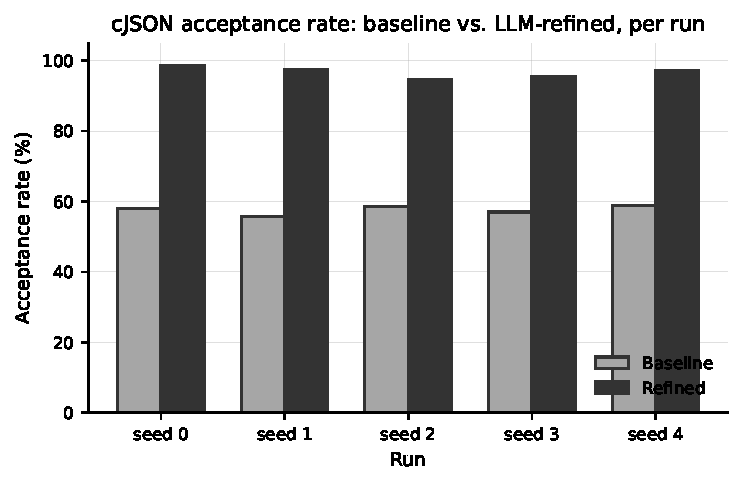
\includegraphics[width=0.85\linewidth]{figures/acceptance_comparison.pdf}
\caption{Per-run acceptance rate, baseline vs.\ refined, cJSON (fifteen
seeded runs per arm). Every refined run exceeds every baseline run.}
\label{fig:acceptance-comparison}
\end{figure}

\textbf{Unequal budgets.} Baseline runs execute 500 inputs on average;
refined runs execute 1{,}533 on average, because each refined run has up
to five iterations of 500 inputs and an iteration whose LLM proposal is
rejected executes none (29 of the 75 refined iterations). Every
count-based quantity (accepted, rejected, fingerprints, signatures as raw
totals rather than rates) therefore scales with a budget that differs
between arms and is not directly comparable; acceptance rate is scale-free
and unaffected by this. We report the budget-sensitive metrics above as
\emph{sums over a run's iterations} specifically so the comparison is
transparent about this rather than implying parity.

\textbf{No crashes in either arm.} Zero sanitizer crashes, timeouts, or
fatal signals occurred in either arm across all thirty runs. The effect
measured here is therefore on generator quality -- validity and structural
diversity -- not on vulnerability discovery in cJSON; we do not claim or
imply that refinement found, or was likely to find, a memory-safety bug in
this target.

\subsection{RQ2: replication on parson}
\label{sec:evaluation-parson}

We reused every pipeline component unchanged against a second, independent
target, parson~\cite{gabis2024parson} (commit \texttt{ba29f4e}, v1.5.3); only
the harness differs.
Reconciling the same JSON grammar against parson's real behavior surfaced
three adaptations, two of which go the \emph{opposite} direction from the
cJSON adaptations reported in Section~\ref{sec:methodology} under the
identical grammar: (i) unlike the cJSON harness, parson's parse entry point
does not require full-buffer consumption, so trailing garbage after a valid
value is silently accepted -- a superset of what the grammar's
\texttt{json : value EOF ;} production specifies; (ii) parson explicitly
rejects any object containing a duplicate key, propagating the rejection up
as a failure for the whole object -- a subset of what cJSON accepts, even
though the grammar itself is silent on duplicate keys for both; (iii) parson
enforces a fixed nesting limit (\texttt{MAX\_NESTING = 2048}), rejecting
deeper structures outright rather than exhibiting unbounded recursion. That
the same formal grammar under-determines a directly opposite validity
decision (duplicate keys: accept vs.\ reject) on two independently
implemented parsers is, on its own, evidence that a purely formal grammar
specification cannot supply the target-specific signal needed to fuzz either
implementation precisely.

\textbf{Replication.} Table~\ref{tab:parson} reports the pre-registered
replication of RQ1's design on parson. Refinement \emph{lowered} acceptance:
92.4\% against the baseline's 95.6\% (exact two-sided Mann--Whitney
$p \approx 0.024$, Cliff's $\delta = -0.48$). The baseline has tied values,
which the exact test assumes away; a tie-corrected test ($p \approx 0.025$)
and a permutation test on the difference in means ($p \approx 0.005$) agree.
No crash, timeout, or signal occurred in 25{,}500 sanitizer-instrumented
executions, and 39 of the 75 refined iterations lost their proposal to
sandbox validation (29 of 75 on cJSON).

\begin{table}[t]
\centering
\footnotesize
\caption{parson: baseline vs.\ LLM-refined, fifteen seeded runs per arm,
identical design to Table~\ref{tab:cjson-comparison}. $p$: exact two-sided
Mann--Whitney U on per-run acceptance rate.}
\label{tab:parson}
\begin{tabular}{@{}lrr@{}}
\toprule
Metric & Baseline & Refined \\
\midrule
Acceptance rate, mean (sd) & 95.61\% (0.95) & 92.41\% (3.96) \\
Acceptance rate, per-run range & 94.0--97.0\% & 86.7--98.7\% \\
Crashes / timeouts / signals & 0 & 0 \\
Distinct rejection signatures & 1 & 1 \\
\midrule
\multicolumn{3}{@{}l}{Refined $-$ baseline: $-3.20$ pp, $p \approx 0.024$, $\delta = -0.48$} \\
\bottomrule
\end{tabular}
\end{table}

\textbf{Why refinement lowers acceptance on parson.} Every input parson
rejected in either arm is explained by a construct confirmed with a minimal
document against the harness. The baseline alternates a grammar-valid
document with the same document plus one trailing suffix (a comma, a bracket,
a brace, a word, or a NUL byte). cJSON's full-buffer entry point rejects every
suffix except NUL, which is what gives it room to improve; parson accepts any
bytes after a complete value, so none is rejected, and its only baseline
rejections (329 of 7{,}500) are objects whose key contains an escaped NUL,
which parson's source states it does not support. The baseline therefore
starts at 95.6\% with almost nothing for refinement to fix. The refined
generators are more varied and produce grammar-valid constructs that parson
refuses. Of the 1{,}063 inputs it rejected, 474 contain a duplicate key, 427
an unpaired surrogate escape, 138 a number that overflows a double, 136 a
zero followed directly by an exponent (\texttt{0e5}), and 10 a NUL in a key
(an input can have several); only 6 are not valid under the grammar. The
last two numeric cases differ in status: RFC~8259 permits limits on number
range, but \texttt{0e5} is valid JSON, and support for it was proposed to
parson and not merged~\cite{parsonpr188}. A further 392 inputs (2.2\%)
failed to encode and count as not accepted, as in RQ1. Finally, parson's
parser returns no error detail, so all 1{,}392 rejections in both arms share
one rejection signature: the proxy tells the proposer how many inputs failed,
never why.

\subsection{Exploratory parson pilot}
\label{sec:evaluation-parson-pilot}

Before API access was available, an exploratory pilot ran five iterations on
parson whose proposals were not produced by the loop's LLM proposer: they
were written outside the loop, in an interactive session with an AI coding
assistant that could read parson's source code. The pilot is therefore
neither LLM-proposer-driven nor black-box, and we report it only for what it
targeted and found, not as evidence about the method.
Table~\ref{tab:parson-iterations} summarizes its iterations.

\begin{table*}[t]
\centering
\caption{parson, exploratory pilot (not part of the statistics): five iterations of 500 examples each, with proposals written outside the loop.}
\label{tab:parson-iterations}
\small
\begin{tabularx}{\textwidth}{c X r r}
\toprule
Iter.\ & Focus (abridged) & Acc./Rej.\ & Fingerprints \\
\midrule
1 & Grammar-seeded generator: recursion, numeric edge cases, duplicate keys, trailing garbage & 285 / 215 & 206/500 \\
2 & Wide objects/arrays (up to 4000 keys) to hit rehash/resize paths unreached by iter.\ 1 & 341 / 159 & 273/500 \\
3 & Hash-bucket collisions, combined wide+deep structures, surrogate escapes at closing quote & 442 / 58 & 254/500 \\
4 & Internal error-cleanup free path: structures valid until the final token & 85 / 415 & 214/500 \\
5 & Combines iter.\ 4's free-path shapes with a sibling-cascade free case & 139 / 361 & 302/500 \\
\bottomrule
\end{tabularx}
\end{table*}

No crash was found in the pilot's 3{,}000 sanitizer-instrumented
executions (500 baseline plus $5 \times 500$ pilot iterations), verified
by grepping every run's stderr for AddressSanitizer, UndefinedBehaviorSanitizer,
and LeakSanitizer text and checking for any non-\texttt{accepted}/\texttt{rejected}
status. A source review of the highest-risk code paths -- \texttt{parse\_utf16}'s
raw pointer walk across surrogate pairs, \texttt{process\_string}'s
output-buffer sizing, \texttt{json\_object\_grow\_and\_rehash}'s linear
probing, and, informed specifically by iterations 4--5, \texttt{json\_object\_add}'s
duplicate-key failure branch and \texttt{parse\_object\_value}/\texttt{parse\_array\_value}'s
missing-bracket failure branch -- found that each relies on the harness's own
null terminator as a safe, in-bounds stopping condition, and that internal
cleanup calls to \texttt{json\_value\_free} are consistent with the harness's
own top-level call (an object's key count is never incremented before a
duplicate is detected, so cleanup never iterates past the last successfully
added slot). We report this as a defensible, evidence-supported explanation
for the absence of a crash within this budget, not as proof that none
exists: five iterations against one pinned commit, exercising the parse and
internal free paths but not parson's public mutation API
(\texttt{json\_object\_remove}, \texttt{json\_array\_remove}, and the
\texttt{\_replace\_*} family), is a bounded search, and we do not claim more
than that bound supports.

\subsection{RQ3: which feedback signal drives the improvement}
\label{sec:evaluation-ablation}

Table~\ref{tab:ablation} reports the feedback-signal ablation described in
Section~\ref{sec:methodology}: the same refined-arm recipe run under each of
the three feedback modes, five seeded trials (seeds 0--4) per mode. In one
trial per mode, all five refinement iterations produced an LLM proposal that
failed sandbox validation (Section~\ref{sec:methodology}), leaving that
trial with no executed inputs; these three trials are excluded, leaving four
usable trials per mode -- the same proposal-rejection behavior visible
throughout RQ1's refined arm, just concentrated into a full trial in these
smaller-sample runs rather than spread across otherwise-successful trials.

\begin{table*}[t]
\centering
\caption{cJSON refined arm under three feedback modes, four usable seeded
trials per mode (one trial per mode excluded; see
Section~\ref{sec:evaluation-ablation}). Descriptive only: with $n{=}4$ per
condition and no separation between conditions, no significance test is
reported or implied.}
\label{tab:ablation}
\begin{tabular}{lrrr}
\toprule
Feedback mode & Acceptance rate & Fingerprints (sum/run) & Rej.\ signatures (sum/run) \\
\midrule
\texttt{counts} & 92.58\% & 505.5 & 6.5 \\
\texttt{counts+rejections} & 96.42\% & 457.3 & 26.8 \\
\texttt{full} & 95.53\% & 503.5 & 34.8 \\
\bottomrule
\end{tabular}
\end{table*}

All three modes raise acceptance rate to a broadly similar, near-ceiling
level -- exposing only acceptance/rejection counts is already close to
sufficient for that specific objective, and the per-trial acceptance rates
across modes overlap (Table~\ref{tab:ablation}), so we do not claim any mode
is statistically distinguishable from another on this metric at $n{=}4$.
The one pattern worth reporting descriptively is rejection-signature
diversity, which increases monotonically with how much of the signal the
proposer sees: \texttt{counts} alone, with no visibility into which
rejection shapes are already covered, produces under a fifth of the
distinct rejection signatures that \texttt{full} feedback does, consistent
with -- though not proof of -- the concern raised in
Section~\ref{sec:discussion} that a proposer optimizing acceptance rate
without visibility into rejection diversity has less reason to keep
producing malformed, boundary-probing input. At four trials per condition,
this is a suggestive, small-sample result, not a tested effect, and we
report it as exactly that.

\section{Discussion}
\label{sec:discussion}

\subsection{Interpreting the effect on cJSON}
The result in Section~\ref{sec:evaluation} says something narrower than ``the
LLM makes fuzzing better'': across fifteen seeded runs, refinement reliably
moved a generator from producing mostly-invalid input toward producing
mostly-valid input, using only the three coverage-free proxies it was given.
That acceptance-rate effect is real and statistically clean at the sample
size tested -- the scale-free metric on which the two arms are directly
comparable -- but it is worth being explicit about what it does not show.
A 97.1\% mean acceptance rate is close to a ceiling, and a
generator that always emits valid input has, by construction, stopped
exercising the accept/reject boundary at all -- exactly the region the
project's own \texttt{near\_valid\_json} baseline strategy exists to probe.
Acceptance rate rising is desirable when the baseline is far from valid and
mostly testing the rejection path, which is the regime our baseline started
in; it is not obviously desirable in the limit, where a generator that never
produces a rejected or malformed input has traded away exactly the
boundary-probing behavior that historically finds parser bugs. We did not
observe this failure mode directly -- within the refined arm, structural
fingerprint counts also rose and rejection signatures did not collapse to a
single trivial case, though these counts are descriptive rather than
tested against the baseline (Section~\ref{sec:evaluation}) -- but the proxy
signal as designed rewards acceptance rate monotonically and has no
explicit floor protecting the near-valid regime.
A refinement objective that also rewarded a target reject rate, rather than
treating ``more accepted'' as strictly better without limit, would be a
direct, low-cost improvement to the design evaluated here.

\subsection{Interpreting the parson result}
The replication shows that the acceptance proxy depends on the target in two
ways. First, it needs headroom: a baseline built from trailing-byte mutations
is almost fully accepted by a parser that ignores trailing bytes, so there is
little left for refinement to raise. Second, it needs the target to be strict
in the places the grammar is, and to say why it rejects: parson refuses
grammar-valid constructs that cJSON accepts and reports no error detail, so a
proposer shown only counts and a single rejection signature cannot tell that
its duplicate keys or \texttt{0e5} numbers are the problem. Refinement then
turns the concern raised above for cJSON around: its more varied generators
reach more of the grammar, and on this target that costs acceptance. For
fuzzing this is not wasted effort, since those inputs exercise parson's
rejection paths, but it means acceptance rate cannot serve as the objective
on its own, and it motivates a proxy that separates grammar-valid rejections
from malformed input.

Finding no crash in 25{,}500 sanitizer-instrumented executions on parson, and
none in the exploratory pilot, is evidence about this pipeline's search within
this budget on this pinned commit, not evidence about parson's correctness in
general. It cannot distinguish ``no bug in the code paths we exercised'' from
``a bug exists in a code path we did not exercise,'' such as parson's public
mutation API, which the black-box parse-then-free harness used here cannot
reach at all.

What the parson runs do establish is narrower and more mechanical: every
non-target-specific pipeline component (\texttt{runner}, \texttt{campaign},
\texttt{proposal}, \texttt{refinement}, \texttt{triage}, \texttt{minimize})
worked unmodified against a second parser with a different, and in several
respects opposite, set of grammar adaptations, with only a new harness and
build script required. The pipeline is portable across targets; the effect
of its acceptance proxy is not.

\subsection{Threats to validity}
\textbf{Construct validity.} A ``crash'' in this pipeline is defined purely
by sanitizer output and process signals; it cannot detect a parser that
silently misparses, accepts input the grammar disallows, or otherwise
violates the specification without a memory-safety fault. The grammar
mismatches documented in Sections~\ref{sec:methodology}
and~\ref{sec:evaluation} (duplicate keys, full-buffer consumption) were
found by deliberately generating inputs in that region and reading the
result, not by any automated oracle; a generator that never targets an
under-specified region of the grammar would not surface this class of
finding at all.

\textbf{Internal validity.} The parson replication ran 24 days after the
cJSON runs, with the harness rebuilt by Homebrew clang 23.1 because a
toolchain upgrade had removed the clang 22 sanitizer runtime it was linked to;
acceptance depends on parson's parsing logic, not on the sanitizer runtime,
and every binary is identified by hash in its run's reproducibility report.
The structural-fingerprint proxy truncates at
256 bytes (Section~\ref{sec:methodology}), so it systematically undercounts
diversity among longer, deeply nested inputs -- exactly the inputs a
refinement loop chasing ``more diversity'' is most likely to produce over
successive iterations, which could understate the true diversity signal
reflected in the descriptive fingerprint counts we report.

\textbf{Statistical validity.} $n{=}15$ runs per arm is still modest; the
exact test used is appropriate for that size and makes no distributional
assumption, but $p \approx 1.29\times10^{-8}$ on the acceptance-rate
comparison is a ceiling on how small an exact $p$-value fifteen-per-arm
observations can produce, not a measure of effect size on its own, and we report the actual
acceptance-rate numbers, alongside the descriptive fingerprint and
rejection-signature counts, in Table~\ref{tab:cjson-comparison} for that
reason. Baseline and refined arms also executed different total numbers of
inputs (Section~\ref{sec:evaluation}), which is why only the scale-free
acceptance rate is tested statistically; any reader extending this
comparison with new count-based metrics should convert to a rate first.

\textbf{External validity.} All results are on JSON, on two relatively
small and independently well-tested C parsers, with one LLM
(\texttt{gpt-4.1-mini}) at one temperature setting for every LLM-driven
arm. The two parsers already disagree on the direction of the effect; we make
no claim that either magnitude, or the absence of a crash, generalizes to
other formats, other parsers, or other proposer models.

\subsection{When this approach is, and is not, the right tool}
The motivating case for a coverage-free feedback loop is a target that
genuinely cannot be instrumented -- a vendored dependency pinned at a
specific commit for compatibility reasons, a license-restricted or
closed-source binary, or a cross-compiled/embedded parser where an
instrumented build would not be representative of what ships. Where
coverage instrumentation \emph{is} available, a coverage-guided or
grammar-aware coverage-guided fuzzer (Section~\ref{sec:related-work}) has
strictly more signal to work with and should be preferred; this pipeline is
not proposed as a replacement for that setting, only as an option for the
black-box one.

\subsection{Future work}
Several extensions are direct given the existing infrastructure. First, the
feedback-signal ablation in Section~\ref{sec:evaluation-ablation} was run at
a small scale (four usable trials per mode) and its rejection-signature
finding is reported descriptively for that reason; a larger-sample
replication is the natural next step to establish whether the pattern we
observed holds statistically. Second, adding an explicit reject-rate floor
to the refinement prompt, motivated directly by this section's concern about
an acceptance-rate ceiling and now further motivated by the ablation's
rejection-signature pattern, could test whether it preserves
boundary-probing behavior without sacrificing the acceptance-rate gain
measured here. Third, and most directly relevant to parson, driving
\texttt{json\_value\_free} through parson's public mutation API rather than
only the parse-then-free path would exercise object lifetime code this
black-box harness cannot currently reach at all. Fourth, comparing against
an existing external fuzzer under an equalized time or execution budget,
rather than only against this project's own static baseline, is the most
direct way to situate the magnitude of the cJSON result against prior work.

Two further extensions are larger in scope and deliberately left for future
work rather than attempted here. One is broadening beyond a second
same-language, same-format target: a third C JSON parser would add little
to what the parson replication already shows about target dependence, whereas a
target in a different format, or a memory-safe language where a
``crash'' oracle must be redefined around uncaught exceptions and API
contract violations rather than sanitizer output -- for instance, JSON
deserialization in a Dart/Flutter mobile application -- would test
generalization along a materially different axis than implementation alone.
The other is applying this pipeline to a live, running mobile or server
application rather than a bounded harness process, which would require
redesigning the outcome-classification step in
Section~\ref{sec:methodology} around that environment's own failure
signals.

\section{Conclusion}
\label{sec:conclusion}

We asked whether an LLM, given only a formal grammar and the feedback a
black-box harness can actually produce -- acceptance rate, structural
diversity, and rejection signatures, with no coverage instrumentation at
all -- can iteratively refine a grammar-based fuzzing generator. Across
fifteen seeded runs against a pinned cJSON build, it reliably can: mean
acceptance rate rose from 58.2\% to 97.1\% relative to a static baseline,
with complete rank separation between arms in this scale-free outcome.
Structural fingerprints and rejection signatures were useful within-campaign
feedback signals, but their aggregate counts are not treated as cross-arm
effects because the arms used different budgets. A feedback-signal ablation
found that acceptance-rate gains hold up under a sparser signal than the
full one, but that the full signal preserves more rejection-signature
diversity -- a small-sample, descriptive finding that motivates, without yet
proving, an explicit reject-rate objective as future work. Reusing the same
pipeline, unmodified, against a second, independently adapted target
(parson) confirmed the mechanics generalize across targets, while five real
refinement iterations and 3{,}000 sanitizer-instrumented executions found no
crash -- a result we reported as an explainable negative finding, supported
by manual review of the highest-risk code paths, rather than reframed as a
success.

The broader point this project argues for is methodological rather than a
single number: a coverage-free proxy signal, cheap enough to compute from a
black-box harness's own accept/reject decision, is sufficient to steer
LLM-guided refinement of a grammar-based generator, which matters
specifically for the targets coverage-guided fuzzing cannot reach -- pinned
vendored dependencies, closed or license-restricted binaries, and embedded
or cross-compiled parsers. We also found that reconciling a formal grammar
against two real, independently implemented parsers is itself informative:
the same grammar under-specifies a directly opposite validity decision
(duplicate object keys accepted by one implementation, rejected by the
other) on two targets, which is exactly the kind of target-specific
knowledge a purely formal specification cannot supply and that fuzzing
against the real implementation surfaces for free.

We release the full pipeline, both harnesses, every campaign artifact, and
the reproducibility tooling described in Section~\ref{sec:methodology}, so
that the comparison in Section~\ref{sec:evaluation} and the null result on
parson can both be checked, extended, or falsified directly rather than
taken on faith.\footnote{\url{\artifacturl}}


\section*{Acknowledgment}
\textbf{Use of generative AI.} An AI coding assistant, Claude
Code~\cite{anthropic2026claudecode}, was used throughout this work: to
implement the harnesses and pipeline, to run and analyze the experiments, and
to draft and revise the text of every section. The OpenAI model named in
Section~\ref{sec:methodology} is the system under study, not a writing aid.
The author directed the work, reviewed all content, and takes full
responsibility for it.


\bibliographystyle{IEEEtran}
\bibliography{references}

\end{document}
